\documentclass{article}
\title{Making Packages in R}
\date{March 3rd, 2023}


\usepackage{geometry}
    \geometry{
        a4paper,
        margin=20mm,
    }

\usepackage{hyperref}
\hypersetup{
    colorlinks=true,
    urlcolor=blue,
    }

\usepackage{graphicx}

\usepackage{xcolor}
\usepackage{xparse}

\NewDocumentCommand{\code}{v}{%
\texttt{\textcolor{purple}{#1}}%
}

\setlength{\parindent}{0pt}

\begin{document}

\maketitle

Notes for the R Package Workshop on 2023-03-03.

\section{Pre-work}

\begin{enumerate}
    \item \textbf{Install R}

        If you already have R, note your version with \code{R --version} in a terminal or typing \code{R.version} in an R console (like in RStudio).
        If you are getting R for the first time, get version 4.2.2.

        \begin{enumerate}
            \item MacOS: \url{https://cran.rstudio.com/bin/macosx/}
            \item Windows: \url{https://cran.rstudio.com/bin/windows/base/R-4.2.2-win.exe}
        \end{enumerate}

    \item \textbf{Install RStudio:} \url{https://posit.co/download/rstudio-desktop/}

    \item \textbf{Get the R Build toolchain}
        \begin{enumerate}
            \item Windows:

                \begin{itemize}
                    \item Go to \url{https://cran.r-project.org/bin/windows/Rtools/} and begin installing the version that matches your R version
                    \item When installing, make sure ``Edit the system PATH'' is \textbf{unchecked} and ``Save version information to registry'' is \textbf{checked}
                \end{itemize}

            \item MacOS:
                \begin{itemize}
                    \item Register as an Apple developer (for free): \url{https://idmsa.apple.com/IDMSWebAuth/signin?appIdKey=891bd3417a7776362562d2197f89480a8547b108fd934911bcbea0110d07f757&path=%2Fregister%2Fagree%2F&rv=1}
                    \item Open a terminal and type \code{xcode-select --install}
                \end{itemize}
        \end{enumerate}
    
    \item \textbf{Install R packages that help you make R packages}
        \begin{itemize}
            \item Open RStudio
            \item Within the console tab, enter: \newline \code{install.packages(c("devtools", "roxygen2", "testthat", "knitr"))}.
                See picture on the next page for assistance.
        \end{itemize}

    \item \textbf{Move the attached ``em-data'' folder to a location on your laptop that you can find}

        Perhaps in your ``Documents'' folder. Or maybe even, ``Downloads''.
\end{enumerate}

\begin{figure}
\center
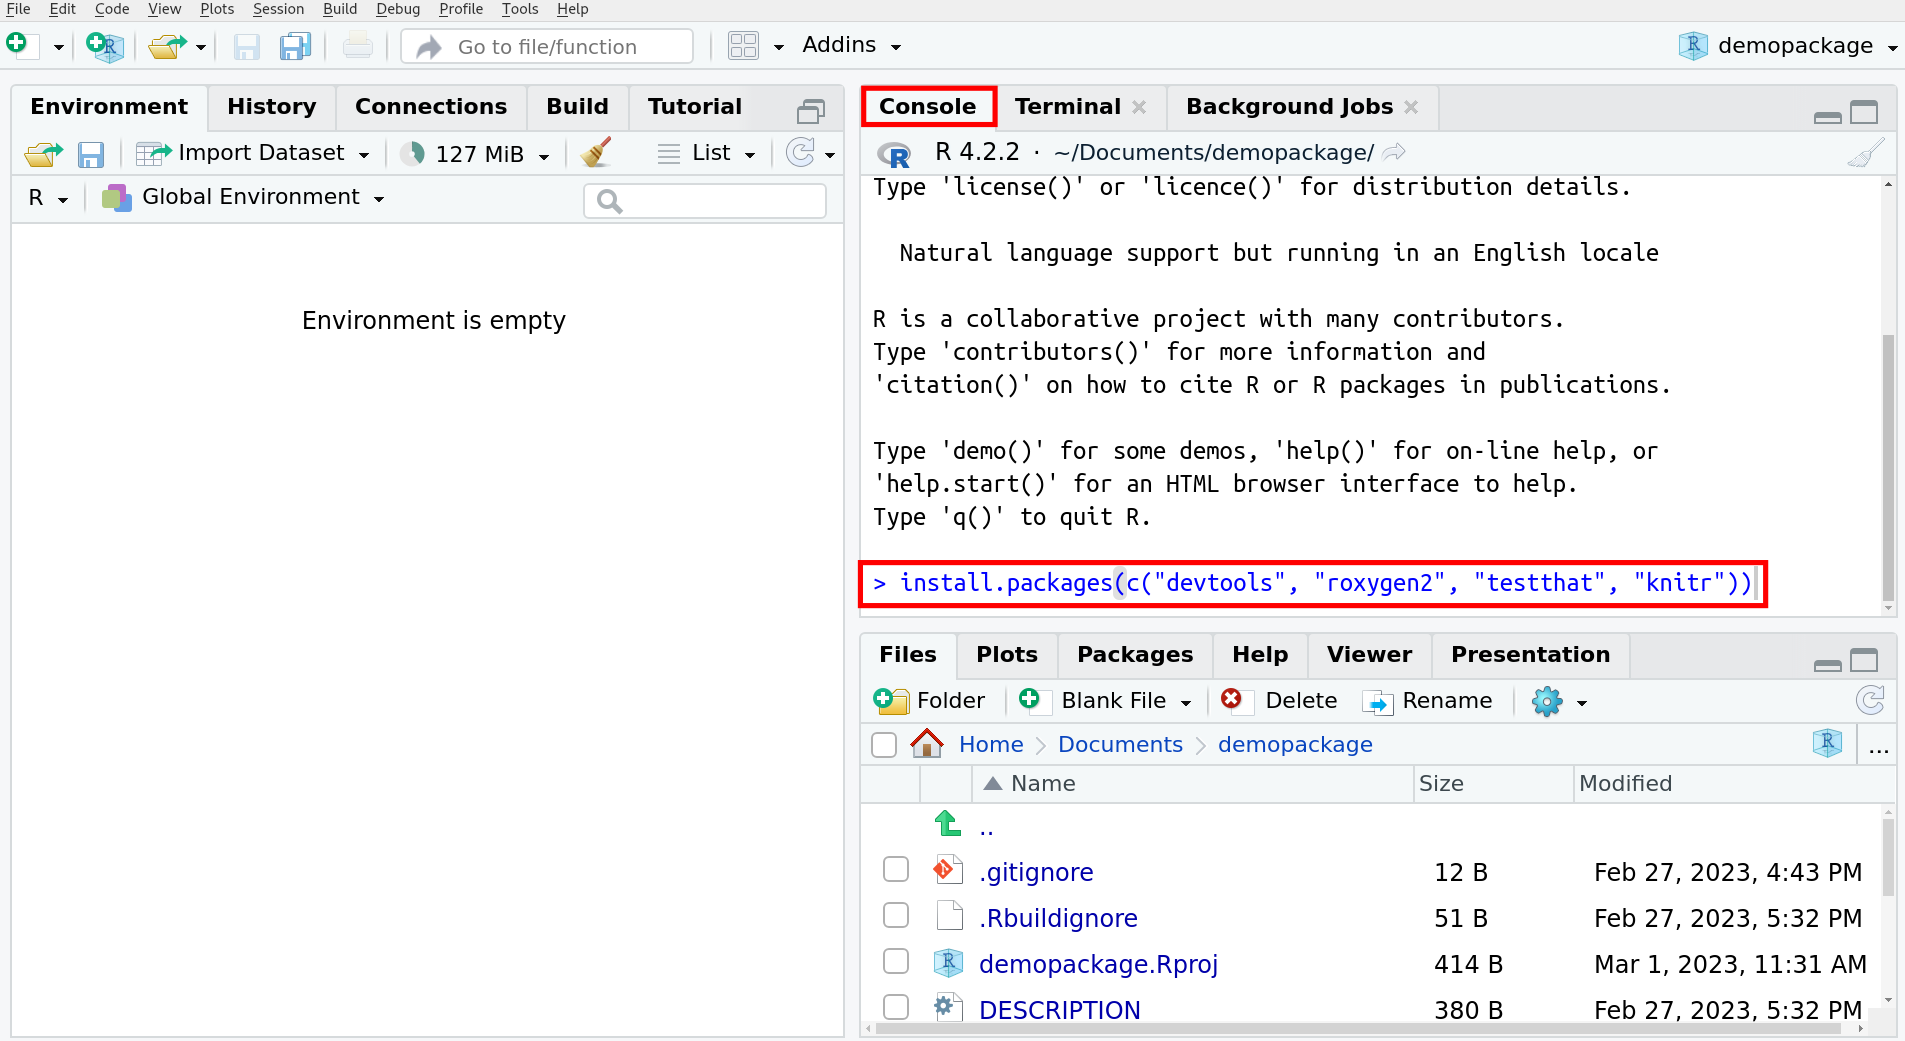
\includegraphics[width=\textwidth]{./install_packages.png}
\end{figure}





\end{document}
